% Este es el fichero EsquemaAlternativo.tex escrito para participar en la 
% IX RESCI que se celebrar\'a en Barcelona conjuntamente la UAB y la UOC.
% Sigue el esquema de publicaci\'on Lecture Notes in Computer Science
% version 2.2 for LaTeX2e
%% Fitxer creat per descriure la debilitat descoberta en el esquema ECElGamal.
%% Fichero 'AnalisisElGamalEccGnuPG-8PostRef.tex', revisado despu�s de los referees de CEDI07
%% Rev.: 11.jun.07

\documentclass{cedi}%llncs}
\usepackage{amsmath,amsfonts,amsthm,amssymb}
\usepackage{pstricks,pst-plot,pst-tree}
%\usepackage[final]{graphicx}
\usepackage{algorithmic,algorithm}
\usepackage[spanish]{babel}

%%% Control de Versiones

%%%%%%%%%%%%%%%%%%%%%%%%%%% VERSIONES %%%%%%%%%%%%%%%%%%%%%%%%%%%%%%%%%%%
\newcommand{\version}{Versi\'on 2.00}
%%%%%%%%%%%%%%%%%%%%%%%%%%%%%%%%%%%%%%%%%%%%%%%%%%%%%%%%%%%%%%%%%%%%%%%%%
% ?? una ' en latex

%%% Abreviaturas

\def\ce{curva{} el\'{\i}ptica}%
\def\ces{curvas{} el\'{\i}pticas}%
\def\CE{Curva{} El\'{\i}ptica}%
\def\CEs{Curvas{} El\'{\i}pticas}%
\def\cf{cuerpo finito}%
\def\cfs{cuerpos finitos}%

%%% Definiciones matem\'aticas especiales

\newcommand{\Z}{\ensuremath{\mathbb{Z}}}%			Enteros
\newcommand{\Q}{\ensuremath{\mathbb{Q}}}%			Racionales
\newcommand{\A}{\ensuremath{\mathbb{A}_{2}}}%			Plano Af\'{\i}n
\newcommand{\Proy}{\ensuremath{\mathbb{P}_{2}}}%		Plano Proyectivo
\newcommand{\K}{\ensuremath{\mathbb{K}}}%			Cuerpo en general
\newcommand{\F}{\ensuremath{\mathbb{F}}}%			Cuerpo finito en general
\newcommand{\Fp}{\ensuremath{\mathbb{F}_p}}%			Cuerpo finito de orden p (primo)
\newcommand{\EFp}{\ensuremath{E(\mathbb{F}_p)}}%		Curva el\'\{i}ptica sobre un cuerpo finito de orden p (primo)
\newcommand{\Fm}{\ensuremath{\mathbb{F}_{2^m}}}%                Cuerpo finito de caractar\'{\i}stica 2, grado m
\newcommand{\Fq}{\ensuremath{\mathbb{F}_q}}%			Idem id. q (q=p^m, p primo y m entero pos.)
\newcommand{\Zn}[1]{\ensuremath{\mathbb{Z}/#1\mathbb{Z}}}%	Anillo de los enteros mod n
\newcommand{\PaI}{\ensuremath{\mathcal{O}}}%                    Punto en el Infinito
\newcommand{\PaIe}{\ensuremath{\mathcal{O}_{E}}}%               Punto en el Infinito de la curva

%%%% ``Castellanizaci\'on'' de 'algorithmic.sty'

\renewcommand{\algorithmicrequire}{\textbf{Prerequisito:}}%
\renewcommand{\algorithmicensure}{\textbf{Postrequisito:}}%
\renewcommand{\algorithmiccomment}[1]{/* #1 */}%	
\renewcommand{\algorithmicend}{\textbf{fin}}%
\renewcommand{\algorithmicif}{\textbf{si}}%
\renewcommand{\algorithmicthen}{\textbf{entonces}}%
\renewcommand{\algorithmicelse}{\textbf{si no}}%
\renewcommand{\algorithmicfor}{\textbf{para}}%
\renewcommand{\algorithmicforall}{\textbf{para todo}}%
\renewcommand{\algorithmicdo}{\textbf{hacer}}%
\renewcommand{\algorithmicwhile}{\textbf{mientras}}%
\renewcommand{\algorithmicloop}{\textbf{bucle}}%
\renewcommand{\algorithmicrepeat}{\textbf{repetir}}%
\renewcommand{\algorithmicuntil}{\textbf{hasta}}%

\floatname{algorithm}{Algoritmo}%

%%% Teoremas y dem\'as
\theoremstyle{plain}        			% Cargar el paquete theorem.sty o amsthm.sty

\theoremstyle{definition}   			% Cargar el paquete amsthm.sty

\newtheoremstyle{saltolinea}% name   		% Sacado del 'thmtest.tex'
  {9pt}%               Space above, empty = `usual value'
  {9pt}%               Space below
  {}%                  Body font
  {}%                  Indent amount (empty = no indent, \parindent = para indent)
%  {\bfseries}%         Thm head font
  {\scshape}%          Thm head font
  {}%                  Punctuation after thm head
  {\newline}%          Space after thm head: \newline = linebreak
  {}%                  Thm head spec

\theoremstyle{saltolinea}   			% Cargar el paquete amsthm.sty
\newtheorem{algo}{Algoritmo}

%%%%%%%%%%%%%%%%%%%%%%%%%%%%%%%%%%%%%%%%%%%%%%%%%%%%%%%%%%%%%%%%%%%%%%%%%%%%%%%%%%%%%%%%%%%%%%%%%%%%%%%
%%% desde llncs.cls para indicar la instituci\'n de la que se forma parte
% LaTeX does not provide a command to enter the authors institute
% addresses. The \institute command is defined here.

\newcounter{@inst}
\newcounter{@auth}
\newcounter{auco}
\newdimen\instindent
\newbox\authrun
\newtoks\authorrunning
\newtoks\tocauthor
\newbox\titrun
\newtoks\titlerunning
\newtoks\toctitle

\def\clearheadinfo{\gdef\@author{No Author Given}%
                   \gdef\@title{No Title Given}%
                   \gdef\@subtitle{}%
                   \gdef\@institute{No Institute Given}%
                   \gdef\@thanks{}%
                   \global\titlerunning={}\global\authorrunning={}%
                   \global\toctitle={}\global\tocauthor={}}

\def\institute#1{\gdef\@institute{#1}}

\def\institutename{\par
 \begingroup
 \parskip=\z@
 \parindent=\z@
 \setcounter{@inst}{1}%
 \def\and{\par\stepcounter{@inst}%
 \noindent$^{\the@inst}$\enspace\ignorespaces}%
 \setbox0=\vbox{\def\thanks##1{}\@institute}%
 \ifnum\c@@inst=1\relax
   \gdef\fnnstart{0}%
 \else
   \xdef\fnnstart{\c@@inst}%
   \setcounter{@inst}{1}%
   \noindent$^{\the@inst}$\enspace
 \fi
 \ignorespaces
 \@institute\par
 \endgroup}

\def\@fnsymbol#1{\ensuremath{\ifcase#1\or\star\or{\star\star}\or
   {\star\star\star}\or \dagger\or \ddagger\or
   \mathchar "278\or \mathchar "27B\or \|\or **\or \dagger\dagger
   \or \ddagger\ddagger \else\@ctrerr\fi}}

\def\inst#1{\unskip$^{#1}$}
\def\fnmsep{\unskip$^,$}
\def\email#1{{\tt#1}}
%%%%%%%%%%%%%%%%%%%%%%%%%%%%%%%%%%%%%%%%%%%%%%%%%%%%%%%%%%%%%%%%%%%%%%%%%%%%%%%%%%%%%%%%%%%%%%%%%%%%%%%
\begin{document}

%%%%%%%%%%%%%%%%%%%%%%%%%%%%%%%%%%%%%%%%%%%%%%%%%%%%%%%%%%%%%%%%%%%%%%%%%%%%%%%%%%%%%%%%%%%%%%%%%%%%%%%
\title{An\'alisis del cifrado ElGamal de un m\'odulo con \ces{} propuesto para el GnuPG}

\author{Sergi Blanch i Torn\'e\inst{1} y Ramiro Moreno Chiral\inst{2}\\ $^1$ Escola Polit\`ecnica Superior, UdL, \email{sblanch@alumnes.udl.cat}\\ $^2$ Departament de Matem\`atica, UdL, \email{ramiro@matematica.udl.cat}}
\date{}

\maketitle
\thispagestyle{empty}

%%%%%%%%%%%%%%%%%%%%%%%%%%%%%%%%%%%%%%%%%%%%%%%%%%%%%%%%%%%%%%%%%%%%%%%%%%%%%%%%%%%%%%%%%%%%%%%%%%%%%%%
\begin{abstract}
Desde marzo de 2007, el paquete de software libre Gnu Privacy Guard (\texttt{GnuPG}) incorpora en la versi\'on de desarrollo soporte para criptograf\'{\i}a con \ces{}. El c\'odigo all\'{\i} incluido fu\'e realizado como proyecto final de carrera del primero de los autores. Sin embargo, y aunque el esquema de firma ECDSA se mantiene en esa versi\'on de desarrollo, el esquema de cifrado \emph{ElGamal} sobre \ces{} presenta algunos problemas que se analizan y se plantea una soluci\'on alternativa como propuesta a la comunidad del \texttt{GnuPG}.
\end{abstract}

\section{Introducci\'on.} 
Hace un tiempo (ver \cite{bm:proyecto,bm:gnupgces}) nos propusimos la implementaci\'on y desarrollo de un m\'odulo de cifrado y firma digitales con \ces{} para incorporarlo al \texttt{GnuPG}. Los algoritmos fundamentales del m\'odulo consist\'{\i}an en un cifrado tipo ElGamal y el conocido algoritmo ECDSA. Se usaron \ces{} definidas sobre cuerpos finitos primos, dadas en la forma reducida de Weierstra\ss{}
\begin{equation}\label{eq:WRF} E/\Fp:\; y^2=x^3+ax+b,\end{equation}
donde $a,b\in\Fp$ y el discriminante $-16(4a^3+27b^2)\ne 0$.

La base normativa del m\'odulo implementado (\cite{P1363,NIST}) da una garant\'{\i}a de seguridad inicial. Pero ya estaba claro que la fase de desarrollo deb\'{\i}a ir avanzando en paralelo con la de an\'alisis. Y gracias a que as\'{\i} ha sido y gracias tambi\'en a la potencia de reflexi\'on y comunicaci\'on que ofrece liberarlo como software libre, se ha visto una debilidad importante en el cifrado ElGamal implementado en el m\'odulo. Como es frecuente, esa debilidad no est\'a causada por el algoritmo en s\'{\i}, sino por el contexto en que se aplica.

El esquema de cifrado ElGamal (cf. por ejemplo \cite[\S{}8.4]{HAC}) sobre un grupo c\'{\i}clico $\mathcal{G}$ cualquiera, con notaci\'on multiplicativa y generador $g$, consiste en usar el intercambio de claves Diffie--Hellman (DH) como una parte de la cifra. As\'{\i}, se calcula $\gamma=g^k$, donde $k$ es una clave de sesi\'on, menor que el orden de $\mathcal{G}$. El mensaje $m$, se convierte en un elemento de $\mathcal{G}$, i.e., $m\in\mathcal{G}$, y se ``esconde'' oper\'andolo en $\mathcal{G}$ con la clave com\'un DH, $\delta=m.(g^a)^k$, siendo $g^a$ la clave p\'ublica del receptor. El mensaje cifrado es el par $(\gamma,\delta)$. El receptor puede recuperar el mensaje ya que $m=\delta(\gamma^a)^{-1}$ y $a$ es su clave privada. Visto el esquema sobre el grupo multiplicativo de un cuerpo finito primo, $\Fp^*$, $m$ ser\'a un entero $1\le m\le p-1$, y la segunda parte del cifrado se calcula mediante productos y potencias m\'odulo $p$,
$$\delta=m.(g^a)^k\mod{p}.$$
En las \ces{} la operaci\'on es la suma y la ``suma abreviada'' $[n]P$ (que se denota simplemente $k\cdot P$) en el grupo de puntos $\EFp$,
$$\delta=m+k\cdot(a\cdot g)\in\EFp,$$
siendo ahora el mensaje y el generador puntos de $\EFp$, es decir $m,g\in\EFp$. La robusted del criptosistema se basa en la del problema Diffie--Hellman: obtener $g^{ak}$ a partir de $g^a$ y $g^k$ en el grupo en que se haya definido.

Pero, al usar \ces{}, aparece una nueva dificultad: representar el mensaje en claro $m$ como punto de $\EFp$. Como se ver\'a no existen soluciones buenas para ello, por lo que se opta por tratarlo como entero $1\le m\le p-1$ y esconderlo modularmente,
$$\delta=m.x(k\cdot(a\cdot g))\mod{p},$$
donde $x(\cdot)$ es la abscisa del punto correspondiente. Pero el tama\~no de $p$ en los criptosistemas con \ces{} es mucho menor que el correspondiente a ElGamal original sobre $\Fp$ (160 bits frente a 1024) y puede pasar que $m>p$ con mucha probabilidad, de modo que al descifrar no se obtenga $m$ sino $m\mod{p}$. Concretamente, en los sistemas \emph{h\'{\i}bridos}, como el \texttt{GnuPG}, en los que se usa un sistema sim\'etrico para cifrar los mensajes largos y un sistema de clave p\'ublica o asim\'etrico, que cifra la clave del sim\'etrico, es normal que $m$ sea precisamente la clave del sistema sim\'etrico. Normalmente, esas claves son \emph{strings} de no m\'as de 256 bits que, al tratarlos como mensajes del criptosistema asim\'etrico, se han de convertir a enteros. Esos tama\~nos resultan ser mayores que el m\'odulo $p$ en un criptosistema con \ces{}. Aumentar el tama\~no de $p$ es renunciar a una de las mayores ventajas de estos criptosistemas: el menor tama\~no de las claves con la misma seguridad de ElGamal sobre cuerpos finitos o del RSA. La soluci\'on podr\'{\i}a ser no hacer modular ese producto, pero entonces, como es p\'ublico, su factorizaci\'on es plausible, revelando as\'{\i} la clave en cuesti\'on.

\begin{figure}\begin{center}
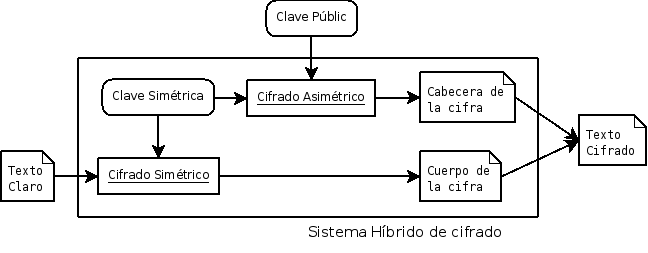
\includegraphics[scale=0.3,clip]{./imgs/sis_hibrido.png}
\caption{Esquema de funcionamiento de un sistema h\'{\i}brido de cifrado.}\label{hibrido}
\end{center}\end{figure}

Es lo que ocurre en nuestra implementaci\'on para el \texttt{GnuPG}, y esa debilidad permite atacar el cifrado asim\'etrico que se realiza a la clave sim\'etrica, con bastantes garant\'{\i}as de \'exito. Hacer este producto modular significa, pues, rechazar toda pretensi\'on de cifrar una informaci\'on cuyo tama\~no sea mayor que el de la clave. Para el caso de un esquema sobre \cfs{} eso no produce ning\'un contratiempo, pues las claves asim\'etricas son mucho mayores que las sim\'etricas. Pero cuando sobre el grupo c\'{\i}clico sobre el que se quiere hacer criptograf\'{\i}a es un subgrupo del $\EFp$, esta diferencia entre sim\'etricos y asim\'etricos conduce peligrosamente a la posibilidad de la factorizaci\'on. Se ha analizado todo ello e ingeniado una soluci\'on de esta debilidad que no deje ninguna limitaci\'on, ni en \'esta ni en posteriores mejoras.

\section{Cifrado tipo ElGamal.} % Visi\'o Abstracta de la debilitat.

El algoritmo de cifrado ElGamal est\'a ampliamente extendido en aplicaciones criptogr\'aficas y multitud de desarrollos, entre otros en el \texttt{GnuPG}. En un sistema de clave p\'ublica, este algoritmo implementa de forma muy eficiente un intercambio de claves Diffie-Hellman para compartir un secreto entre dos comunicandos, con el que, al mismo tiempo, cifra un mensaje. A pesar de que tambi\'en existe un esquema de firma ElGamal, no goza de gran difusi\'on y est\'a superado por el esquema DSA. De hecho, el esquema de firma ElGamal se considera comprometido desde finales de 2000 (ver \cite{insecure}).

Nuestra propuesta es poner a prueba el esquema usado en el cifrado, no s\'olo cuando el esquema o algoritmo ElGamal se usa sobre el grupo de puntos de las {\ces}, sino tambi\'en cuando es utilizado sobre el grupo multiplicativo de los cuerpos finitos, $\Fp^*$. Como veremos, resulta altamente dependiente del tama\~no de $p$, pues es el segundo operando el que plantea el problema del tama\~no del espacio de mensajes o, en su caso, el de factorizaci\'on de enteros (\texttt{IFP}).

\subsection{Esquema cl\'asico ElGamal.}

El siguiente algoritmo~\ref{alg:ElGamal} es el esquema b\'asico de cifrado tipo ElGamal en el grupo $\Fp^*$. Con $pkey_M$ se denota un \emph{registro} que es la clave p\'ublica del usuario $M$. Se supone que tal registro est\'a formado por los siguentes campos

\begin{center}\begin{tabular}{c|l}$pkey_M.p$ & \hspace{1mm} orden del cuerpo finito  \\ \hline $pkey_M.g$ & \hspace{1mm} generador: $\Fp^*=\langle g\rangle$\\ \hline $pkey_M.y$ & \hspace{1mm} clave p\'ublica $y=g^x$,\\[-.5mm] & \hspace{1mm} siendo $x$ la privada\end{tabular}\end{center}

El algoritmo~\ref{alg:ElGamal} recibe, como una componente de la entrada, el mensaje a cifrar que damos en llamar $z$. Hay que destacar que, a pesar de que se trata como un elemento de $\Fp^*$, en nuestra implementaci\'on representar\'a una clave de cifrado sim\'etrico, que originalmente son \emph{strings} de no m\'as de 256 bits.

\begin{algo}[Cifrado ElGamal]\label{alg:ElGamal}
\parbox[b]{\linewidth}{%
\hrule
\smallskip
{\bf INPUT}: Clave p\'ublica $pkey_{M}$ y entero a cifrar $z\in\Fp^*$.

{\bf OUTPUT}: Cifrado formado por un par de enteros, $(a,c)\in\Fp^*\times \Fp^*$.
\vspace{1.5mm}
\hrule
}%
\begin{algorithmic}[1]
\STATE Generar aleatoriamente una clave de sesi\'on $k\in_{R}\left[1,\left(pkey_{M}.p\right)-2\right]$;
\STATE $a=(pkey_{M}.g)^{k}\mod p$;
\STATE $b=(pkey_{M}.y)^{k}\mod p$; \\
\COMMENT{$y=g^x\mod p$; $b=(g^x)^k\mod p$}
\STATE $c=z\cdot b\mod p$;
\STATE Return $(a,c)$;
\end{algorithmic}
\end{algo}%

\subsection*{Estudio del esquema.}

Tal algoritmo basa su robustez en los siguientes hechos,
\begin{itemize}
	\item La aleatorizaci\'on de la clave de sesi\'on (paso~1) lo hace sem\'anticamente seguro y resistente a los cl\'asicos ataques por texto cifrado escogido.
	\item El uso del esquema Diffie-Hellman en los pasos~2 y~3 (el valor $b$ es la clave compartida que no viajar\'a por el canal).
	\item S\'olo resolviendo el DLP (\emph{Discrete Logarithm Problem}) un atacante puede calcular $k$ a partir de $a$. As\'{\i} conseguir\'a el secreto compartido $b$ que se usa para camuflar la informaci\'on a cifrar en el producto $c=z\cdot b\mod p$, que es la operaci\'on ElGamal propiamente dicha y, por lo tanto, el mensaje original $z$
%	\item La dificultad de resolver el IFP (\emph{Integer Factorization Problem}\footnote{Como ya se ha comentado, este problema no se plantea si este paso se hace modular, $c=z\cdot b\mod{p}$. Debe tenerse en cuenta que entonces $z$ no deber\'a ser mayor que $p$.}) en el paso~4. 
\end{itemize}
Sin embargo, como todo esquema b\'asico ElGamal sobre un grupo gen\'erico $\mathcal{G}$, tambi\'en \'este adolece de una deficiencia: la limitaci\'on del espacio de mensajes, ya que $z\in\Fp^*$ (cf. por ejemplo \cite{DHAES}). Esta limitaci\'on es muy importante si el cardinal del grupo es ``peque\~no''.
%Pero tambi\'en puede ser atacado directamente el esquema de ElGamal resolviendo el problema de factorizaci\'on de enteros (IFP) y factorizar $c$. Esta factorizaci\'on deber\'{\i}a ser lo suficientemente dif\'{\i}cil, pero dependiendo de c\'omo sean los factores $z$ y $b$, puede no serlo.

%Las claves usadas comunmente en criptograf\'{\i}a est\'an definidas sobre cuerpos finitos, y las opciones de criptosistema m\'as frecuentes son RSA o ElGamal/DSA. De todos modos, las longitudes de claves sobre cuerpos finitos, como es habitual, siguen creciendo: lo que hace unos a\~nos se consideraba una clave segura, hoy no tiene una longitud suficiente; as\'{\i}, las claves de 1024 bits son ya cosa del pasado: las recomendables han aumentado hasta longitudes de 2048 bits. 
%Esto que parecer\'{\i}a una mejora, puede constituir un problema.

%Fij\'emonos en la operaci\'on de ElGamal. Es un simple producto \textbf{no} modular, cuyos factores son de muy distintos tama\~nos. Efectivamente, el factor que proviene del protocolo de intercambio Diffie-Hellman, tiene una longitud considerable y podr\'{\i}amos decir que s\'olo rompiendo el protocolo lo obtendr\'{\i}amos. Con las longitudes actuales comentadas, ser\'a frecuentemente un valor de 2048 bits.

%El principal problema est\'a en el valor que queremos cifrar, $z$. ?`Qu\'e tama\~no tiene? Al usar sistemas h\'{\i}bridos de cifrado, como el \texttt{GnuPG}, se genera una clave de sesi\'on para cifrar con un sistema sim\'etrico el grueso del mensaje y es esta clave la informaci\'on que ciframos de forma asim\'etrica. Por lo tanto, el tama\~no de ese factor estar\'a entre 128 y 256 bits. Aunque eso constituye una ventaja, ya que ciframos individualmente para cada destinatario un dato relativamente peque\~no, evitando la expansi\'on de bits propia de los sistemas asim\'etricos en el cifrado de todo el mensaje, tambi\'en puede ser una debilidad por la gran diferencia de tama\~no con el otro factor del cifrado. Efectivamente, se puede pensar en una factorizaci\'on de $c$ que busque factores relativamente peque\~nos como son esos valores $z$: tal factorizaci\'on, aunque dif\'{\i}cil, es viable.

%Esa clave de sesi\'on es, pues, nuestro problema. Su origen le da unas caracter\'{\i}sticas muy peculiares, que debilitan el cifrado tipo ElGamal.

\subsection{Esquema El\'{\i}ptico ElGamal: ECElGamal.}

El trabajo original consisti\'o en el desarrollo de un m\'odulo criptogr\'afico con \ces{} definidas sobre cuerpos finitos primos $\Fp$ y su inclusi\'on dentro del \texttt{GnuPG}: uno de nuestros prop\'ositos era hacer llegar el uso generalizado de los criptosistemas sobre \ces{} al p\'ublico no especializado por medio del software libre. Veamos, pues, c\'omo funciona un cifrado de este tipo. En el algoritmo~\ref{alg:ECElGamal} se puede ver la descripci\'on del esquema con \ces{} ECElGamal, que es una ``traducci\'on'' directa del algoritmo~\ref{alg:ElGamal} sobre cuerpos finitos $\Fp$. En este caso los campos de la clave p\'ublica $pkey_M$ son $n$, el orden del grupo de puntos generado por $G$, $n=|\langle G\rangle|$, el propio punto generador $G$, y el punto $P$, clave p\'ublica, tal que $P=d\cdot G$, siendo $d$ un entero que se usa como clave privada.

\begin{algo}[Cifrado ECElGamal]\label{alg:ECElGamal}
\parbox[b]{\linewidth}{%
\hrule
\smallskip
{\bf INPUT}: Clave p\'ublica $pkey_{M}$ y entero a cifrar $z$.

{\bf OUTPUT}: Cifrado formado por un par de puntos, $(R,C)$.
\vspace{1.5mm}
\hrule
}%
\begin{algorithmic}[1]
\STATE Generar aleatoriamente una clave de sesi\'on $k\in_{R}\left[1,\left(pkey_{M}.n\right)-1\right]$;
\STATE $R=k\cdot pkey_{M}.G$;
\STATE $Q=k\cdot pkey_{M}.P$; \\
\COMMENT{$P=d\cdot G$; $Q=k\cdot (d\cdot G)$}
\STATE Convertir el mensaje en punto de la \ce{} $z\rightarrow Z$;
\STATE $C=Z+Q$;
\STATE Return $(R,C)$;
\end{algorithmic}
\end{algo}

La ``traducci\'on'' a \ces{} es sencilla: esencialmente consiste en sustituir el grupo multiplicativo c\'{\i}clico $(\Fp^*,\cdot)$ por un subgrupo c\'{\i}clico $(\mathcal{G},+)=(\langle G\rangle,+)$ del grupo de puntos de la \ce{}, $E(\Fp)$, con lo que
\begin{itemize}
	\item la notaci\'on cambia de multiplicativa a aditiva (productos a sumas, y potencias a productos de puntos por enteros);
	\item el orden del grupo $\mathcal{G}$, ha de ser lo m\'as pr\'oximo posible al del grupo total $E(\Fp)$;
	\item el mensaje $z$ se ha de convertir en punto.
\end{itemize}


\subsection*{Estudio del esquema.}

Este esquema con \ces{}, tiene una clara ventaja: el producto que se usa como operaci\'on b\'asica del cifrado ElGamal sobre $\Fp^*$ y que constituye la debilidad ya indicada, es ahora una suma de puntos $C=Z+Q$ que no se puede ``deshacer'' sin conocer alguno de los sumandos, y eso s\'olo es posible si se resuelven algunos de los ECDLP, \emph{Elliptic Curve Discrete Logarithm Problem}, subyacentes en los pasos 2 y 3 del algoritmo~\ref{alg:ECElGamal}.

Pero la conversi\'on del mensaje $z$ a cifrar en punto $Z\in\EFp$ {\bf no} es trivial. Recordemos que el mensaje a cifrar $z$ es originalmente un \emph{string} de bits que constituye la clave de un sistema de cifrado sim\'etrico, por lo que no se puede hacer ninguna conjetura sobre su estructura. Una vez transformado a un entero $\mod p$, i.e., $z\in\Fp$, se puede considerar candidato a abscisa de un punto de $E(\Fp)$. Pero no siempre resulta $z$ una abscisa de un punto racional de la \ce{} $E/\Fp$: efectivamente, seg\'un la ecuaci\'on~\eqref{eq:WRF}, el valor $z^3+az+b$ ha de ser un cuadrado en el cuerpo base $\Fp$. Si no lo es, hay que hacer alguna transformaci\'on de $z$, $z\mapsto z_1$, tal que el s\'{\i}mbolo de Legendre de $z_1^3+az_1+b$ sobre $p$ sea $1$. Entonces $Z_1=(z_1,y_1)\in\EFp$, donde $y_1$ es una de las dos ra\'{\i}ces cuadradas de $z_1^3+az_1+b$ en $\Fp$. Pero, para poder descifrar, hay que enviar, junto con el par de puntos $(R,Z_1+Q)$, del paso~6 del algoritmo~\ref{alg:ECElGamal}, informaci\'on adicional que permita invertir la transformaci\'on $z\mapsto z_1$.

Aunque se han usado diferentes soluciones para este problema, todas adolecen de un defecto u otro. Y, en general, en todas ellas es pensable que se podr\'{\i}a estar dando informaci\'on adicional sobre el valor de $z$. Por ello se debe descartar este esquema de cifrado.

%Para esta conversi\'on se necesita la equaci\'on~\ref{eq:WRF}, pero no siempre resulta $z$ una abscisa de un punto de $E(\Fp)$, ya que, obviamente, no siempre $z^3+az+b$ es un cuadrado en el cuerpo base $\Fp$. Aunque se han usado diferentes soluciones para este problema, todas adolecen de un defecto u otro. Y, en general, en todas ellas es pensable que se podr\'{\i}a estar dando informaci\'on adicional sobre el valor de $z$. Por ello debemos descartar este esquema de cifrado.

%Para tratar esta conversi\'on, recordemos que \emph{forma} tiene el mensaje a cifrar $z$. Hemos ido repitiendo que a pesar de tratar a esta entrada como un entero de $\Fp^*$, en origen es un \emph{string} de bits de un sistema sim\'etrico. Es decir, no podemos considerarlo como un valor aleatoriamente seguro ni m\'aximo. Lo que significa que no debemos suponerle \emph{a priori} ninguna informaci\'on sobre su forma o estructura.

%Una vez considerado como un entero de $\Fp^*$, podemos considerarlo candidato a abscisa. Ya deciamos que al calcular su ordenada seg\'un la equaci\'on~\ref{eq:WRF} esta puede no ser un cuadrado en el cuerpo base $\Fp$, as\'{\i} que cualquier \emph{truco} que hagamos para convertirlo en algo v\'alido deberemos hacerselo llegar al destinatario por medio de la cifra para deshacer tambi\'en esta conversi\'on. Por ejemplo, buscar un entero $z'$ de $\Fp^*$ cercano a $z$ que si se corresponda con una abscisa v\'alida para establecer un punto $Z'$, nos dar\'a un valor, llamemosle $m : z'=m+z$ con el que en el descifrado deber\'a ser conocido para recuperar la $z$ original.

\section{Esquema ECDH+ElGamal.}

Entendiendo el esquema inicial del algoritmo~\ref{alg:ElGamal} como dos partes separadas, por un lado el intercambio de claves DH y por otro la operaci\'on producto, asociada propiamente al cifrado ElGamal, se puede buscar una soluci\'on al anterior problema. Realizando un intercambio de claves del tipo Diffie-Hellman sobre \ces{}, se obtiene un secreto compartido con el cual llevar a cabo la operaci\'on ElGamal sobre enteros, resultando el algoritmo~\ref{alg:ECDH} descrito a continuaci\'on.

\begin{algo}[Cifrado ECDH+ElGamal]\label{alg:ECDH}
\parbox[b]{\linewidth}{%
\hrule
\smallskip
{\bf INPUT}: Clave p\'ublica $pkey_{M}$ y texto en claro num\'erico $z$.

{\bf OUTPUT}: Punto resultante $R$, cifra $c$.
\vspace{1.5mm}
\hrule
}%
\begin{algorithmic}[1]
\STATE Generar aleatoriamente una clave de sesi\'on $k\in_{R}\left[1,\left(pkey_{M}.n\right)-1\right]$;
\STATE $R=k\cdot pkey_{M}.G$;
\STATE $Q=k\cdot pkey_{M}.P$; \\
\COMMENT{$P=d\cdot G$; $Q=k\cdot (d\cdot G)$}
\STATE $c=z\cdot Q_x\mod p$; \\
\COMMENT{$Q_x$ es la abscisa de $Q$, $Q_x=x(Q)$}
\STATE Return $(R,c)$
\end{algorithmic}
\end{algo}


\subsection*{Estudio del esquema.}

Con este algoritmo se evita la molesta conversi\'on de la informaci\'on a cifrar en punto de la \ce{}, resultando en ese sentido un esquema m\'as simple que el del algoritmo~\ref{alg:ECElGamal}, que estaba implementado usando s\'olo operaciones sobre los puntos de la curva. Pero otra vez aparece el problema ya comentado de la limitaci\'on del espacio de mensajes: para recuperar $z$ ha de ser $z\in\Fp^*$, es decir, $1\le z\le p-1$.

Una primera aproximaci\'on es hacer el producto del paso~4 no modular,
$$\text{4. }c=z\cdot Q_x.$$
Pero la robusted del esquema depende ahora de la dificultad de resolver el IFP (\emph{Integer Factorization Problem}) en ese paso~4. Y en nuestra implementaci\'on esa dificultad es menor de lo habitual. Efectivamente, suponiendo que el intercambio DH el\'{\i}ptico ha de tener una seguridad equivalente a ElGamal 2048 sobre cuerpos finitos (a su vez equivalente a un RSA con m\'odulo de 2048 bits), el orden del grupo de puntos $E(\Fp)$ habr\'{\i}a de ser de unos 256 bits, es decir, el punto $Q$, obtenido en el paso 3, vendr\'a dado por dos coordenadas de ese tama\~no (igualmente el punto $R$ y el punto--clave p\'ublica $P$). La clave de sesi\'on que proviene del cifrado sim\'etrico tendr\'a como m\'{\i}nimo 128 bits. As\'{\i} pues, ese producto no modular, dado como alternativo al del paso 4 del algoritmo~\ref{alg:ECDH}, tendr\'a factores de esos rangos, 128 y 256 bits, y por tanto, un tama\~no final de 384 bits: !`nada dif\'{\i}cil de factorizar para algoritmos modernos como el de la GNFS, \emph{General Number Field Sieve} (\cite{bbfk:rsa640GNFS})!.

Manteniendo el citado paso~4 como producto modular aparecer\'an con frecuencia problemas de los tama\~nos relativos de $z$ y $p$. As\'{\i} ocurrir\'a cuando se use una clave $z$ para el AES256 y un cuerpo base de la \ce{} para el esquema ECElGamal de 192 bits (el menor de los permitidos en la implementaci\'on): ser\'a $z>p$ y, al descifrar, no se recuperar\'a $z$ sino $z \mod p$.

Una situaci\'on como la descrita har\'{\i}a que la ejecuci\'on del \texttt{GnuPG} re\'usase siempre el cifrado. Cabr\'{\i}a pensar que si se ``troceara'' la clave de sesi\'on $z$ que se ha usado en el cifrado sim\'etrico y se procediera a dos cifrados asim\'etricos separados, se resolver\'{\i}a el problema de los tama\~nos relativos. Pero esta grata soluci\'on te\'orica no resulta posible en la pr\'atica de las implementaciones del \texttt{OpenPGP}~\cite{OPGP}: en las m\'as usadas, y una de ellas es el \texttt{GnuPG}, el m\'odulo de cifrado asim\'etrico recibe como entrada un solo \emph{string} de bits y s\'olo puede devolver como salida una cifra de estructura est\'atica; por lo tanto, no es posible decidir cu\'ando no hace falta trocear, y cu\'ando s\'{\i} (en el futuro, incluso podr\'{\i}a no ser suficiente con dos partes). Esta soluci\'on, pues, tambi\'en se queda corta: hay que encontrar algo que resulte m\'as gen\'erico y no obligue a dar soluciones \emph{ad hoc} en cada paso y momento.
%Es decir, tenemos en este caso tama\~nos de los factores m\'as pr\'oximos entre s\'{\i} que los del algoritmo original: si en el estudio del primer esquema~\ref{alg:ElGamal} sobre cuerpos finitos, ten\'{\i}amos una gran distancia entre los operandos del producto, ahora tenemos valores de una longitud similar. Pero estamos en lo mismo, los operandos tienen caracter\'{\i}sticas que les hacen demasiado peculiares.

%Al factorizar el valor $c$ del producto, podemos encontrarnos con dos situaciones extremas. Una en la que ambos factores fuesen primos: se tratar\'{\i}a de factorizar un entero de 384 bits, producto de dos primos de tama\~no similar. No parece una tarea inabordable, sino todo lo contrario: por un lado, estamos realizando un intercambio de claves bastante robusto, mientras que por otro conf\'{\i}amos en una factorizaci\'on de un entero mucho menor de lo que aceptar\'{\i}amos para un RSA. En el otro extremo podemos encontrar unos operandos altamente compuestos, con lo que obtendr\'{\i}amos una amplia lista de factores r\'apidamente (mucho m\'as que en el otro caso). Y la labor mas pesada ahora ser\'{\i}a separar esa lista en dos grupos, uno para obtener un entero de 128 bits y el otro para uno de 256.

%Ya comentabamos al principio que una soluci\'on general para esta situaci\'on pasa por hacer este producto modular. Y ya entonces remarc\'abamos la proximidad entre los valores que intervienen en este producto. En un caso muy normal, en que se use para el sistema asim\'etrico una \ce{} de 256 bits y para la parte sim\'etrica un AES256 o mayor, hay que rechazar la implementaci\'on de la operaci\'on modular. Sin tener en cuenta la utilizad criptogr\'afica de confrontar los algoritmos como en la situaci\'on propuesta, es f\'acil que ocurra que el valor num\'erico de la clave sim\'etrica sea mayor que el orden del \cf{}.

\section{Esquema alternativo ECDH + AES256.}

Llegados a este punto, se ha de aceptar que el esquema ElGamal no sirve para los prop\'ositos expuestos. Implementado con s\'olo operaciones en el grupo de puntos $\EFp$, como en el algoritmo~\ref{alg:ECElGamal}, aparecen soluciones poco recomendables y no hay seguridad de que el truco usado para convertir el mensaje en punto est\'e revelando informaci\'on a un criptoanalista. La operaci\'on producto ElGamal m\'odulo $p$ har\'a el mensaje irrecuperable, dado el peque\~no tama\~no de $p$. Y, el punto medio consistente en el intercambio de claves en \ces{} y la operaci\'on producto no modular, resulta fatal para el prop\'osito de seguridad criptogr\'afica.

S\'olo queda buscar una alternativa completa a la operaci\'on ElGamal. Hay que seguir pensando en una operaci\'on con enteros, como en el algoritmo~\ref{alg:ECDH}, pues recuperar algo del algoritmo~\ref{alg:ECElGamal} nos llevar\'{\i}a de nuevo al problema de la conversi\'on del mensaje en punto de la \ce{}. Parece que lo m\'as sensato es pensar en una operaci\'on que sustituya al producto, pero de robustez garantizada. Se da como soluci\'on alternativa una operaci\'on basada en un cifrado sim\'etrico. El secreto compartido que genera la parte ECDH, cumple con el ideal de una clave de sesi\'on: nunca viaja por el canal y es conocido por ambos participantes l\'{\i}citos de la comunicaci\'on. Se puede ver este nuevo esquema en el algoritmo \ref{alg:AES}.

\begin{algo}[Cifrado ECDH+AES]\label{alg:AES}
\parbox[b]{\linewidth}{%
\hrule
\smallskip
{\bf INPUT}: Clave p\'ublica $pkey_{M}$ y texto en claro num\'erico $z$.

{\bf OUTPUT}: Par punto resultante $R$ y cifra $c$.
\vspace{1.5mm}
\hrule
}%
\begin{algorithmic}[1]
\STATE Generar aleatoriamente una clave de sesi\'on $k\in_{R}\left[1,\left(pkey_{M}.n\right)-1\right]$;
\STATE $R=k\cdot pkey_{M}.G$;
\STATE $Q=k\cdot pkey_{M}.P$; \\
\COMMENT{$P=d\cdot G$; $Q=k\cdot (d\cdot G)$}
\STATE $c=\textrm{aes256}(z,\{\textrm{sha256}(Q_x)\})$;
\STATE Return $(R,c)$;
\end{algorithmic}
\end{algo}

Conviene aclarar la notaci\'on usada en el paso~4 anterior: con $c=\textrm{aes256}(z,\{\textrm{sha256}(Q_x)\})$ se quiere significar que $c$ es el cifrado obtenido mediante un AES256 del valor $z$, al usar como clave de ese cifrado sim\'etrico $\{\textrm{sha256}(Q_x)\}$.

Este esquema fu\'e propuesto inicialmente en \cite{MMR}. No s\'olo se trata de sustituir la operaci\'on descartada por un cifrado sim\'etrico, sino de evitar futuros errores. Al usar el AES se garantiza la seguridad de este esquema mediante la del AES, intensa y regularmente analizado en la actualidad. Ante un hipot\'etico caso en el que el criptosistema AES se vea comprometido, la soluci\'on pasa por fortalecerlo o incluso llegar a usar otro esquema m\'as robusto. En este mismo sentido se propuso a la P1363a del IEEE, como alternativa a los cifrados tipo ElGamal, un esquema m\'as general que el aqu\'{\i} desarrollado, por parte de Abdalla, Bellare y Rogeway, \cite{DHAES}. Como ya se ha se\~nalado, en esa propuesta se subrayan algunas debilidades de los cifrados ElGamal: la limitaci\'on del espacio de mensajes es la que aparece como definitiva en los cifrados con \ces{} en sistemas h\'{\i}bridos.

M\'as all\'a de esta concreci\'on, es de desear un algoritmo vers\'atil, eficiente y que proporcione un espacio de mensajes sin demasiadas restricciones. Como medida adicional hay introducir una funci\'on de resumen, $\textrm{sha256}$, para as\'{\i} obtener siempre una clave de cifrado sim\'etrico de la misma longitud, que sea m\'axima y que tambi\'en podr\'a ser calculable al descifrar, seg\'un se advierte en el esquema de descifrado propuesto en el algoritmo~\ref{alg:descifrado}.

\begin{algo}[Descifrado ECDH+AES]\label{alg:descifrado}
\parbox[b]{\linewidth}{%
\hrule
\smallskip
{\bf INPUT}: Clave secreta $skey_{M}$ y el par punto resultante $R$ y cifra $c$.

{\bf OUTPUT}: Texto en claro num\'erico $z$.
\vspace{1.5mm}
\hrule
}%
\begin{algorithmic}[1]
\STATE $Q=skey_{M}.d\cdot R$;
\STATE $z=\textrm{aes256}^{-1}(c,\{\textrm{sha256}(Q_x)\})$;
\STATE Return $(z)$;
\end{algorithmic}
\end{algo}

En este caso $skey_{M}$ representa la estructura de clave secreta que contiene los campos de la clave p\'ublica adem\'as del campo $skey_{M}.d$ que es el entero que se usa como clave privada. Y, al igual que al cifrar, la expresi\'on $z=\textrm{aes256}^{-1}(c,\{\textrm{sha256}(Q_x)\})$ indica la recuperaci\'on de $z$ al descifrar $c$ mediante el AES256 con la misma clave $\{\textrm{sha256}(Q_x)\}$.

\subsection*{Estudio del esquema.}

Los algoritmos que se han expuesto como soluci\'on presentan la seguridad basada en el ECDLP y en la del AES y garantizan diferentes niveles de seguridad, que se especifican a continuaci\'on.
\begin{itemize}
	\item La aleatoriedad de la clave de sesi\'on $k$, permite seguridad sem\'antica y resistencia a los ataques por texto cifrado elegido.
	\item No son posibles los ataques de \cite{insecure} ya que el cifrado ElGamal propiamente dicho ha desaparecido: no existe la cl\'asica operaci\'on producto de este tipo de cifrados.
	\item Y, lo que parece m\'as importante en los sistemas h\'{\i}bridos, el espacio de mensajes no tiene limitaciones de tama\~no: las claves sim\'etricas $z$ se cifran con AES.
\end{itemize}

\section{Conclusi\'on}

Se ha visto como el esquema ElGamal se ve comprometido, no por su dise\~no sino por el caso particular en el que se aplica y se ha podido encontrar una alternativa que parece resolver el compromiso. Un esquema ampliamente utilizado ha quedado puesto en duda, y esta duda afecta al m\'as importante de sus usos: los algoritmos h\'{\i}bridos, donde el texto a cifrar es una clave de sesi\'on con la que se ha cifrado sim\'etricamente el grueso de la informaci\'on.

La soluci\'on aportada presenta una gran ventaja, ya que el AES es un criptosistema muy generalizado y constantemente puesto a prueba. Actualmente el algoritmo AES esta bajo presi\'on (\cite{OHT05,BERN05}) debido a que durante este pasado a\~no han aparecido nuevos puntos de partida para el criptoanalisis. Se trata de ataques eminentemente inform\'aticos que aprovechando peque\~nos detalles del ordenador, consiguen hacerse con informaci\'on \'util del cifrado. Por el momento, tiene un impacto comparable al producido por el riesgo de almacenar una frase de paso en la memoria de intercambio de disco.

Habr\'a que estar muy pendientes de la evoluci\'on de estos ataques y en especial de las contramedidas (\cite{OST05}) que se den contra ellos. Por el momento, no se han propuesto soluciones factibles a nivel de la aplicaci\'on. Tan s\'olo existe alguna propuesta, mas o menos aplicable, para ofrecer una protecci\'on desde el sistema operativo o incluso desde la arquitectura del ordenador.

%%%  END  %%%


%%%%%%%%%%%%%%%%%%%%%%%%%%%%%%%%%%%%%%%%%%%%%%%%%%%%%%%%%%%%%%%%%%%%%%%%%%%%%%%%%%%%%%%
%% Bibliograf\'{\i}a

%\bibliographystyle{amsalpha}
%\bibliographystyle{amsplain}
%\bibliography{tesis}

\providecommand{\bysame}{\leavevmode\hbox to3em{\hrulefill}\thinspace}
\providecommand{\MR}{\relax\ifhmode\unskip\space\fi MR }
% \MRhref is called by the amsart/book/proc definition of \MR.
\providecommand{\MRhref}[2]{%
  \href{http://www.ams.org/mathscinet-getitem?mr=#1}{#2}
}
\providecommand{\href}[2]{#2}
\begin{thebibliography}{BM04}

%\bibitem[wp]{wp} \textit{Wikipedia: \texttt{ElGamal} encryption}.
\bibitem[DHAES]{DHAES} M. Abdalla, M. Bellare and P. Rogeway, \textit{DHAES: An encryption scheme based on the Diffie-Hellman Problem}, Submission to IEEEE P1363a, 1999.
\bibitem[OST05]{OST05} D. Arne Osvik, A. Shamir and E. Tromer, \textit{Cache attacks and countermeasures: the case of AES}, 2005.
\bibitem[BBFK05]{bbfk:rsa640GNFS} F.~Bahr, M.~Boehm, J.~Franke, and T.~Kleinjung, \emph{{RSA640 factored by GNFS}}, {\tt NMBRTHRY @LISTSERV. NODAK. EDU}, November 2005.
\bibitem[BERN05]{BERN05} D. Bernstein, \textit{Cache-timing attacks on AES}, 2005.
\bibitem[BM04]{bm:gnupgces} S.~Blanch and R.~Moreno, \emph{Implementaci\'on {GnuPG} con curvas el\'{\i}pticas}, Avances en Criptolog\'{\i}a y Seguridad de la Informaci\'on. Proceedings {RECSI VIII}, 2004, pp.~515--526.
\bibitem[BMTFC]{bm:proyecto} S.~Blanch and R.~Moreno, \emph{GnuPG Implementation with Elliptic Curves}, Trabajo final de carrera, EPS, Universid de Lleida, Marzo 2004.
\bibitem[BJN]{insecure} D. Boneh, A. Joux and P.Q. Nguyen, \textit{Why textbook ElGamal and RSA encryption are insecure}, Proceedings of Asiacrypt'00, Lecture Notes in Computer Science, no. 1976 (2000), Springer, pp. 30-43.
\bibitem[BRUM03]{BRUM03} D. Brumley and D. Boneh, \textit{Remote timing attacks are practical}, 2003.
\bibitem[AES99]{AES99} J. Deamen and V. Rijmen, \textit{AES Proposal: Rijndael, version 2}, AES submission, 1999.
\bibitem[P1363]{P1363} IEEE P1363 Standard Specifications for Public key Cryptography. 2000 January 30.
\bibitem[RFC2440]{OPGP} J. Callas, L. Donnerhacke, H. Finney, R. Thayer, \emph{Request for Comments: 2440; OpenPGP Message Format} November 1998.
\bibitem[KSWH98]{KSWH98} J. Kelsey, B. Scheneier and D. Warner, Chris Hall, \textit{Side channel cryptanalysis of product ciphers}, 5th European Symposium on Research in Computer Security, LNCS 1485, 97-110, Sptinger-Verlag, 1998.
\bibitem[HAC]{HAC} A. J. Menezes,  P. C. van Oorschot  and  S. A. Vanstone, \textit{Handbook of Applied Cryptography}, Fifth Printing (August 2001).
\bibitem[MMR]{MMR} M.~Mylnikov, Comunicaci\'on personal, Noviembre de 2004.
\bibitem[NIST197]{NIST197} National Institute of Standards and Technology, \textit{Advanced Encryption Standard (AES) (FIPS PUB 197)}, 2001.
\bibitem[NIST186-2]{NIST} National Institute of Standards and Technology, \textit{Digital Signature Standard (DSS) (FIPS PUB 186-2)}, 2000 January 27.
\bibitem[NIST180-2]{NIST180-2} National Institute of Standards and Technology, \textit{Secure Hash Standard (SHS) (FIPS PUB 180-2)},2002.
\bibitem[OHT05]{OHT05} M. O'Hanlon and A. Tonge, \textit{Investigation of cache-timing attacks on AES}, 2005.
\bibitem[NFS]{NFS sieving} A. Shamir and E. Tromer, \textit{Special-Purpose hardware for factoring: the NFS sieving step}, 2005.

\end{thebibliography}

\end{document}
